\documentclass[a4paper,12pt,one side,titlepage]{report}

%en francais
\usepackage[T1]{fontenc}
\usepackage[utf8]{inputenc}
\usepackage[francais]{babel}
%fonts
\usepackage{lmodern}
\usepackage[scaled]{helvet}
\usepackage{fourier}
\usepackage{inconsolata}


\usepackage{amsfonts}
\usepackage{amsmath}
\usepackage{amssymb}
\usepackage{eurosym}
\usepackage{float}
%\usepackage[bottom=2.5cm,left=2.5cm,right=2.5cm]{geometry}
\usepackage[bottom=2.8cm]{geometry}
\usepackage{graphicx}
\usepackage[acronym]{glossaries}
\usepackage[hidelinks]{hyperref}
\usepackage{lipsum}
\usepackage{lastpage}
\usepackage{listings}
\usepackage{pdfpages}
%\usepackage{titlesec}
\usepackage{url}
\usepackage{wrapfig}

\graphicspath{ {../images/} } % dossier img

%lstdefines etc....
\lstset{literate=
{á}{{\'a}}1 {é}{{\'e}}1 {í}{{\'i}}1 {ó}{{\'o}}1 {ú}{{\'u}}1
{Á}{{\'A}}1 {É}{{\'E}}1 {Í}{{\'I}}1 {Ó}{{\'O}}1 {Ú}{{\'U}}1
{à}{{\`a}}1 {è}{{\`e}}1 {ì}{{\`i}}1 {ò}{{\`o}}1 {ù}{{\`u}}1
{À}{{\`A}}1 {È}{{\'E}}1 {Ì}{{\`I}}1 {Ò}{{\`O}}1 {Ù}{{\`U}}1
{ä}{{\"a}}1 {ë}{{\"e}}1 {ï}{{\"i}}1 {ö}{{\"o}}1 {ü}{{\"u}}1
{Ä}{{\"A}}1 {Ë}{{\"E}}1 {Ï}{{\"I}}1 {Ö}{{\"O}}1 {Ü}{{\"U}}1
{â}{{\^a}}1 {ê}{{\^e}}1 {î}{{\^i}}1 {ô}{{\^o}}1 {û}{{\^u}}1
{Â}{{\^A}}1 {Ê}{{\^E}}1 {Î}{{\^I}}1 {Ô}{{\^O}}1 {Û}{{\^U}}1
{œ}{{\oe}}1 {Œ}{{\OE}}1 {æ}{{\ae}}1 {Æ}{{\AE}}1 {ß}{{\ss}}1
{ç}{{\c c}}1 {Ç}{{\c C}}1 {ø}{{\o}}1 {å}{{\r a}}1 {Å}{{\r A}}1
{€}{{\EUR}}1 {£}{{\pounds}}1
}

\lstdefinestyle{python}
{
language=python,
numbers=left,
numberstyle=\tiny,
backgroundcolor=\color{yellow!20},
keywordstyle=\color{blue!50!green!50}\bfseries,
commentstyle=\color{black},
stringstyle=\color{red},
showstringspaces=false,
basicstyle=\small\color{blue},
captionpos=b,
tabsize=2,
frame=tb,
breaklines=true
columns=fullflexible,
linewidth=0.9\linewidth,
xleftmargin=0.1\linewidth
}

\lstdefinestyle{ruby}
{
language=ruby,
numbers=left,
numberstyle=\tiny,
backgroundcolor=\color{brown},
keywordstyle=\color{blue!50!green!50}\bfseries,
commentstyle=\color{black},
stringstyle=\color{red},
showstringspaces=false,
basicstyle=\inco\color{blue},
captionpos=b,
tabsize=2,
frame=tb,
breaklines=true
columns=fullflexible,
}

\lstdefinestyle{code}{
%language=bash,
numbers=left,
numberstyle=\tiny\color{black},
basicstyle=\inco\color{white},
%basicstyle=\inco\color{black},%for printing
numbersep=3pt,
frame=tb,
breaklines=true
columns=fullflexible,
backgroundcolor=\color{black},
%backgroundcolor=\color{white},%for printing
%linewidth=0.9\linewidth,
%xleftmargin=0.1\linewidth
}


\definecolor{blocs}{HTML}{0066FF}
\definecolor{plugins}{HTML}{CC0000}
\definecolor{special}{HTML}{CCFF33}

\lstdefinestyle{logstash}{
language=bash,
numbers=left,
numberstyle=\tiny\color{black},
basicstyle=\inco\color{white},
%basicstyle=\inco\color{black},%for printing
backgroundcolor=\color{black},
%backgroundcolor=\color{white},%for printing
keywordstyle=\color{blocs},
keywordstyle=[2]\color{plugins},
keywordstyle=[3]\color{special},
numbersep=3pt,
frame=tb,
breaklines=true
columns=fullflexible,
morekeywords={input,filter,output},
morekeywords=[2]{stdin,stdout,grok,syslog},
morekeywords=[3]{fromage},
commentstyle=\color{purple},
captionpos=b
}


\renewcommand{\familydefault}{phv}
%\renewcommand{\familydefault}{\ttdefault}

\newcommand{\selv}{%
\fontfamily{phv}\fontseries{b}\fontsize{8}{20}\selectfont}
\newcommand{\belv}{%
\fontfamily{phv}\fontseries{b}\fontsize{10}{22}\selectfont}
\newcommand{\inco}{%
\fontfamily{\ttdefault}\fontseries{b}\fontsize{10}{10}\selectfont}
\newcommand{\ipath}[1]{{\inco \normalsize {#1}}}

%%% header & footer
% \leftmark : afficher nom section
\usepackage{fancyhdr}
\pagestyle{fancy}
\renewcommand{\headrulewidth}{1pt}
\fancyhead[C]{\selv\leftmark}
\fancyhead[L]{\selv ELK}
\fancyhead[R]{\selv Équipe réseau Lothaire}%\includegraphics[width=60px]{openstack-logo.png}}

\renewcommand{\footrulewidth}{0pt}
\fancyfoot[C]{\belv Page \thepage\hspace{2px} / \pageref{LastPage}} 
\fancyfoot[L]{
\includegraphics[height=20px]{elasticmini.png}}
\fancyfoot[R]{\belv François \textsc{Dupont}}



%Titre et Auteurs
%\title{Architecture pour l'hébergement web à fort trafic}
%\author{Auteurs : \textit{Dupont Francois}\\\\Tuteur : \textit{Vincent Delove}}
%\date{Lundi 23 Mars 2015}


\newglossaryentry{API}{name={API},
                             description={Une API, Application Programming Interface, est une interface permettant d'interagir avec un programme par l'intermédiaire d'"opérations simples". Elles sont en générale la pour faciliter la réutilisation d'un programme plus complexe. C'est parce que openstreetmap à une API que l'on a vu autant de logiciels utilisant ses cartes/tuiles.
}}

\newglossaryentry{cron}{name={cron},
                             description={Cron est un gestionnaire de tâche automatique sur linux, il est extremement répendu.
}}
\newglossaryentry{flag}{name={flag},
                             description={Un drapeau, dans la dénomination logstash, le flag représente une option passé en argument exemple : -w.
}}

\newglossaryentry{cluster}{name={cluster},
                             description={Cluster ou grappe. Un cluster est constitué d'un ou plusieurs nodes qui partagent le même \emph{cluster.name}
}}

\newglossaryentry{document}{name={document},
                             description={Un document, dans la terminologie elasticsearch, est constitué d'un ou plusieurs nodes qui partagent le même \emph{cluster.name}
}}

\newglossaryentry{fulltext}{name={fulltext},
                             description={Un drapeau, dans la dénomination logstash, le flag représente une option passé en argument exemple : -w.
}}

\newglossaryentry{Munin}{name={Munin},
                             description={Munin est un logiciel de monitoring populaire et simple d'installation
}}

\newglossaryentry{index}{name={index},
                             description={Un index dans la terminologie est ce qui se rapproche d'une base dans le modèle relationnel \emph{classique}. 
}}

\newglossaryentry{lucene}{name={lucene},
                             description={Apache Lucene 
}}
\newglossaryentry{logs}{name={logs},
                             description={Trace (informations) provenant d'un programme ou d'un équipement, souvent sous forme de texte
}}

\newglossaryentry{mapping}{name={mapping},
                             description={Le mapping. Dans la terminologie elasticsearch, un node est processus java 
}}

\newglossaryentry{node}{name={node},
                             description={Node ou noeud est, dans la terminologie elasticsearch, un processus  processus java lucene, c'est une instance d'elasticsearch. 
}}

\newglossaryentry{shard}{name={shard},
                             description={Dans la terminologie elasticsearch, un shard est un index ou un morceau d'index. C'est un index au sens lucene du terme. Il existe deux types de shards, des shards primaires et des shards répliqués. Un shard primaire peut indexer de nouvelles données alors qu'un shard repliqué sert seulement de failover, il peut également être utilisé pour accélérer les réponses aux requêtes.
}}


\newglossaryentry{thread}{name={thread},
                             description={explication thread processus etc.. 
}}

\newglossaryentry{type}{name={type},
                             description={Un type dans la terminologie elasticsearch est l'équivalent d'une table dans le modèle relationnel. Il est équivalent dans la mesure où il possède des champs contenant des valeurs
}}

%\newglossaryentry{BGP}{name={BGP},
%                             description={BGP, Border Gateway Protocle, est un protocole d'échange de routes utilisé sur internet, il permet aux AS (autonomous systems) d'échanger leurs informations.\\
%                             Le plus connu des mauvais usages de BGP s'est produit en février 2008 lorsque Pakistan Telecom a mal appliqué une demande de censure de YouTube, le rendant indisponible pour le monde entier pendant plusieurs heures.\\
%                             Le black-holing BGP est une technique d'endiguement de DDOS souvent utilisée en dernier recours. Pour protéger l'infrastructure réseau (d'un FAI par exemple), on décide que tous les accès à une IP/un range d'IP seront redirigés vers NULL. }}
%\newglossaryentry{CLI}
%{
%	name={CLI},
%	description={Command Line Interface: interface en ligne de commande, se dit d'un programme auquel on accède par l'intermédiaire d'un shell (terminal en ligne de commande). Ces programmes sont en général légers puisqu'ils sont entièrement textuels.}
%}
%
%\newglossaryentry{DDOS}{name={DDOS},
%                        description={Distributed Denial Of Service ou attaque par déni de service distribué. Attaque informatique ayant pour objectif de rendre indisponible un service, un site web etc... en saturant le serveur qui l'héberge (il existe de nombreux type de DDOS différents)}}
%
%\newglossaryentry{firewall}{name={firewall},
%                             description={Pare-feu : système de protection réseau pour un ordinateur ou un réseau d'ordinateur, dans ce projet nous parlerons essentiellement de pare-feu logiciel}}
%
%\newglossaryentry{failover}
%{
%	name={failover},
%	description={Un failover, traduit par passer outre à la panne, est la capacité d'un équipement à basculer automatiquement vers un réseau alternatif ou en veille.}
%}
%
%\newglossaryentry{jumbo frames}{ name={jumbo frames},
%                                description={En réseau, des jumbos frames sont des trames Ethernet dont la longueur dépasse 1500 octets. En général, les jumbo frames peuvent avoir une longueur allant jusqu'à 9000 environ octets.}
%}
%
%\newglossaryentry{hash}
%{
%	name={hash},
%	description={On nomme fonction de hachage une fonction particulière qui, à partir d'une donnée fournie en entrée, calcule une empreinte servant à identifier rapidement, bien qu'incomplètement, la donnée initiale. Les fonctions de hachage sont utilisées en informatique et en cryptographie.}
%}
%
%\newglossaryentry{load balancer}{ name={load balancer},
%                                description={Un répartisseur de charge, ou load balancer, est un ensemble de techniques permettant de distribuer la charge de travail entre plusieurs ordinateurs d'un groupe}
%}
%
%\newglossaryentry{naxsi}
%{
%	name={naxsi},
%	description={Un type de firewall}
%}
%
%\newglossaryentry{OSI}{ name={OSI},
%                                description={Open System Interconnection model est un modèle conceptuel qui caractérise et standardise les communications sur internet. Ce modèle a été standardisé dans l'ISO/IEC 7498-1 (International Organization for Standardization). Il possède 7 couches. 
%                                Réparties comme suit :\\
%    \begin{tabular}{|c|c|c|}
%        \hline
%        Numéro& Couche       & Exemple de protocole\\
%        \hline
%        7&      Applications &  HTTP, NFS, DHCP, BGP, DNS etc... \\
%        \hline
%        6&      Présentation &  MIME, SSL\\ 
%        \hline
%        5&      Session      &  Sockets, SOCKS, NetBIOS\\
%        \hline
%        4&      Transport    & TCP, UDP\\
%        \hline
%        3&      Réseau       & IP4/6, IPsec\\
%        \hline
%        2&      Liaison      & PPP, Token Ring, CRC,\\
%        \hline
%        1&      Physique     & Wifi, Ethernet, CAN, RS-232\\
%        \hline
%    \end{tabular}
%                                }
%}
%
%\newglossaryentry{overhead}
%{
%	name={overhead},
%	description={Coût supplémentaire engendré pour atteindre un but (cette définition est agnostique à la méthode ou la technologie).\\
%    Exemple : Envoyer "Bonjour" à un correspondant par internet (disons sur un chat en ligne), ici la charge utile est "Bonjour"\\
%    Une fois le message enregistré il va être encapsulé de nombreuses fois (TCP, HTTP, conversion en binaire pour la couche physique, etc..)
%    pour être affiché chez notre correspondant. Tout cela prend du temps de calcul, du temps de transport, de la "place" (envoyer toutes
%    ces en-têtes multiplie plusieurs fois la taille du message original). La différence entre le payload (la charge utile originale) et le
%    résultat final est appelé overhead.
%    }
%}
%
%\newglossaryentry{scalabiliser}{ name={scalabiliser},
%                                description={Scalabiliser est un anglicisme courant signifiant mettre à l'échelle. On parle de mise à l'échelle lorsqu'une infrastructure a la capacité de démultiplier sa capacité de traitement. On attend en général que cette mise à l'échelle soit rapide, voire automatisée.}
%}
%
%\newglossaryentry{SSL}
%{
%	name={SSL},
%	description={Secure Socket Layer est un protocole de sécurité SSL qui fonctionne suivant un mode client-serveur. Il permet de satisfaire aux objectifs de sécurité suivants :\begin{itemize}
%	\item l'authentification du serveur.
%	\item la confidentialité des données échangées (ou session chiffrée).
%	\item l'intégrité des données échangées.
%	\end{itemize}
%    voir aussi \gls{TLS}}
%}
%
%\newglossaryentry{TLS}
%{
%	name={TLS},
%	description={Transport Layer Security est une évolution du protocole SSL : cf \gls{SSL}}
%}
%
%\newglossaryentry{wireshark}
%{
%	name={wireshark},
%	description={Wireshark est un analyseur de paquets libre utilisé dans le dépannage et l'analyse de réseaux informatiques, le développement de protocoles, l'éducation et la rétro-ingénierie. Wireshark permet d'analyser les paquets qui transitent sur un réseau en les interceptant.}
%}
%
%
%
%
%
%
%parser


\makeglossaries

\begin{document}

\begin{titlepage}
\begin{center}
 \newcommand{\HRule}{\rule{\linewidth}{0.5mm}}

%
\includegraphics[width=0.15\textwidth]{debian.png}~\\[1cm]

\includegraphics[width=0.55\textwidth]{Logo-IUT-UL.jpg}\hfill

\includegraphics[scale=0.8]{lothaire.jpg}
\vspace{1cm}

\textsc{\large Licence ASRALL}
\vspace{0.5cm}

% Title
\HRule \\[0.4cm]
{ \Large \bfseries Analyse de logs avec ELK\\[0.4cm] }

\HRule \\[1.0cm]

% Author and supervisor
\noindent
\begin{minipage}{0.5\textwidth}
\begin{flushleft} \large
\emph{Auteur:}\\
François \textsc{Dupont}\\
%\Letter~test@exemple.com\\
\end{flushleft}
\end{minipage}%
\begin{minipage}{0.5\textwidth}
\begin{flushright} \large
\emph{Tuteur:} \\
Vincent \textsc{Delove}
\end{flushright}
\end{minipage}

%
\vspace{1cm}

\begin{figure}[h]
    \centering
    
\includegraphics[scale=0.6]{elasticsearch.png}
    \hfill
    
\includegraphics[scale=0.5]{logstash.png}
    \hfill
    
\includegraphics[scale=1]{kibana.png}
    \\[20mm]
    
\includegraphics[scale=0.5]{elastic.png}
\end{figure}

\vspace{3mm}
% Bottom of the page
Stage effectué à la \textbf{Sous Direction des Infrastructures}\\rue du Doyen Marcel Roubault, 54500 \textsc{Vandoeuvre lès Nancy}\\
{Compilé le \today}\\[5mm]%Lundi 23 Mars 2015}
Année Scolaire \textbf{2014-2015}%Lundi 23 Mars 2015

\end{center}
\end{titlepage}




%Page remerciments
\emph{\Large Remerciements}
\\[2cm]
Remerciment 1
\\[1cm]
Remerciment 2
\\[2cm]
Remerciment 3


%Page table des matières
\setcounter{tocdepth}{1}
\tableofcontents

%%%%%%%%%%%%%%%%%%%%%%%%%%%%%%%%%%%%%%%%%%%%%%%%%%%%%%%%%%%%%%%%%
%Introduction
\part{Introduction}

\section{Problématique}
La gestion de \gls{logs} est une problématique commune à presque tous les services informatique,
tous les fournisseurs de services et plus globalement, toutes personnes gérant une infrastructure 
informatisée.

Les \gls{logs} sont précieux car ils sont un des éléments indispensable au dépanage, au monitoring,
à l'anticipation de problèmes inhérant à l'exploitation d'une infrastructure informatique.
\footnote{terme volontairement très vaste}
\emph{De nombreuses structures continuent encore aujourd'hui d'analyser plus ou moins "manuellement" leurs
\emph{\gls{logs}}, qu'ils proviennent de \emph{hardware, ou de software}}.

L'objectif de ce projet est de répondre à la problématique de la gestion et de l'analyse de log, en utilisant
la stack ELK\footnote{Elasticsearch Logstash Kibana}.
Dans ce rapport nous expliquerons de façon plus précise en quoi consiste la gestion de log,
les fonctions et fonctionnement des outils dont nous ferons usage, enfin, nous détaillerons notre 
architecture et ses évolutions possibles.



\chapter{La gestion de logs}

La gestion des \gls{logs} est un problème presque aussi vieux que l'informatique.
Au commencement 

La tendance est cependant (et depuis longtemps) à la centralisation de ces fichiers afin de faciliter 
leur accès et leur analyse ultérieur. Cela permet également une sauvegarde plus facile de ces derniers 
dans le cas où cela est nécessaire. Il est fréquent d'avoir des scripts analysant 
quotidiennement ces \gls{logs} afin de pouvoir détécter un comportement suspect.


\lipsum
\chapter{Les clusters}

\lipsum

\chapter{MoM}

\lipsum
\lipsum

\chapter{Gestion de projet}
\lipsum
%\section{Tableau de bord}

\begin{table}[h]
\begin{tabular}{|*{7}{c|}}
\hline
\multicolumn{7}{|c|}{Tableau de bord}                                  \\\hline
\textbf{\#} & Lundi & Mardi & Mercredi & Jeudi & Vendredi & Commentaires \\\hline
1 & \multicolumn{3}{c}{\textbf{Découverte du projet}}& & $\times$ &
Participation à la réunion d'équipe\\ Installation de ma machine perso \\ Découverte de l'infrastructure réseau \\\hline
2       &       &       &          &       &          &              \\\hline
3       &       &       &          &       &          &              \\\hline
4       &       &       &          &       &          &              \\\hline
5       &       &       &          &       &          &              \\\hline
6       &       &       &          &       &          &              \\\hline
7       &       &       &          &       &          &              \\\hline
8       &       &       &          &       &          &              \\\hline
9       &       &       &          &       &          &              \\\hline
10      &       &       &          &       &          &              \\\hline
11      &       &       &          &       &          &              \\\hline
12      &       &       &          &       &          &            \\\hline 
\end{tabular}
\caption{Tableau de bord}
\centering
\end{table}

\section{Nos objectifs}
\lipsum
\chapter{Présentation des notions}
\chapter{Définitions}

\part{Les logiciels}
\chapter{Logstash}
\begin{figure}[H]
\center

\includegraphics[width=0.2\textwidth]{logstash.png}
\label{fig:logstashlogo.png}
\end{figure}
\section{Présentation de Logstash}

Logstash permet de traiter et/ou de transférer des données, en masse. Dans notre 
projet, nous l'utiliserons essentiellement en conjonction avec Elasticsearch en 
utilitaire de sorti. Cependant,
et comme le montre la liste des ses abondants plugins d'output, Logstash est capable
de fonctionner avec de nombreux autres logiciels.

\subsection{Pourquoi Logstash?}
Bien qu'un administrateur système compétent soit capable d'analyser de façon rapide 
et efficace les logs d'une machine (à l'aide deperl+awk+sed+tail+grep), cette méthode
est fastidieuse. De plus, face à des dizaines/milliers de machines (virtuelles aussi), 
cette méthode n'est plus applicable, elle ne peut pas passer à l'échelle.
Il est actuellement fréquent (cloud, applications multicouche, \ldots) que les logs 
d'une seule machine ne suffise plus à diagnostiquer le problème auquel on est confronté.

\subsection{Fonctionnement interne}
L'utilisation de logstash est un pipeline qui s'articule autour de 3 \emph{blocs} 
également appelés \emph{stages} (phase).
\begin{itemize}
    \item   Le bloc : \emph{Inputs} génère des événements à partir des informations reçues
    par logstash en entrée.
    \item   Le bloc : \emph{Filters} modifie, manipule, ces évènements dans logstash
    \item   Le bloc : \emph{Outputs} envoie les évènements de logstash vers leur 
    prochaine destination.
\end{itemize}

Cette façon de fonctionner peut faire penser à \emph{iptables}.

Logstash est un logiciel développé en Jruby\footnote{sauf mention contraire, on supposera
dans ce rapport que logstash est développé en ruby} (Jruby est en faite une implémentation
de ruby 1.8 en Java qui était à l'époque plus rapide que ruby "seul"). 
Le passage d'une phase à l'autre est implémenté via les \emph{SizedQueue} de ruby. 
Elles sont dimensionnées pour contenir 20 éléments\footnote{appelés messages lorsqu'on parle de queues, on parle bien ici 
des \textbf{événements} logstash}, ce n'est pas paramétrable sans modifier le code 
source, c'est un choix délibéré. Ces queues ne sont pas conçues pour stocker des 
données à long terme. On verra plus tard que ce la justifie l'utilisation d'un 
\textit{buffer}, comme \emph{Redis}\footnote{voir la sous partie sur la tolérence
de pannes ainsi que le chapitre consacré à Redis}.


Chaque bloc est composé d'une multitude de plugins. Ce sont des modules indépendants
qui peuvent également fonctionner en conjonction les uns des autres.

Il est, par exemple, possible de configure le bloc \emph{inputs} pour utiliser 
plusieurs fois le plugin "file" (on imagine pour des cas d'utilisation différents) 
et de se servir dans le même temps d'un autre plugin du bloc \emph{inputs} : stdin 
qui prendra typiquement en entrée le clavier.


Il est possible d'implémenter de nouveaux plugins en ruby afin de les ajouter à
notre logstash.

Il existe également un \textit{pseudo-bloc} qui peut s'insérer dans les autres, ce 
bloc, \emph{codec} permet la de gérer la \textit{représentation des données} c'est 
à dire qu'un codec est capable de lire ou d'écrire dans une syntaxe particulière 
comme par exemple rubydebug, collectd, ou, bien plus intéressant pour nous, netflow.

%wtf why?
%et les types ??


%Explications supplémentaires sur les filtres
% les plugins et les patterns par défaut?

\subsubsection{Tolérance de pannes}
Vos logs sont \textbf{importants}, c'est la raison d'être de Logstash, il ne souhaite 
pas que vous en perdiez le moindre à cause d'un problème réseau ou d'une défaillance
quelconque rendant la destination indisponible.
%cf pipeline.rb et base.rb dans github
Lors d'une indisponibilité, les plugins outputs tentent de renvoyer les événements 
vers leur destination. Si ce n'est pas possible le plugin arrête de lire sa queue 
tant que le message n'a pas pu être envoyé. Par effet domino, une fois la queue 
\textit{filtre => output} remplie, le bloc filtre, ne pouvant plus envoyer de nouveaux 
messages à la queue \textit{FO}. Le plugin du bloc filtre va également retenter 
d'envoyer ses messages, et refuser en attendant de lire les nouveaux arrivant dans 
la queue \textit{input => filtre}.
Si cette dernière venait à se remplir c'est le Logstash tout entier qui refuserait de 
traiter de nouvelles informations. Dans le meilleur des mondes, les expéditeurs de
données se comporterais comme logstash et attendraient patiemment que le problème
se résolve, malheureusement cela n'est pas toujours possible, particulièrement dans
nos problématiques d'où l'importance d'un Redis en amont (ou en aval) afin de 
faire tampon.\footnote{Il existe d'autres outils que Redis, (dont ce n'est pas la fonction
principale) pour réaliser ce travail, ils sont plus adapté mais aussi moins documentés
dans leur utilisation avec logstash.}

\subsubsection{Multithread}
Attention ces informations sont pour le moment, \date{Jeudi 16 Avril}, correctes 
mais sont amenées à changer, notamment concernant les outputs.

Chaque plugin input utilise un \gls{thread}, cela permet d'éviter les engorgements si  
certaines entrées sont plus longues à traiter que d'autres.

En le bloc filtre entier n'utilise par défaut qu'un seul thread, mais il est possible 
d'augmenter le nombre de threads affectés au traitement des filtres avec le \gls{flag}
-w lors du démarrage de Logstash.

À l'heure actuelle le bloc output de logstash ne peut utiliser qu'un seul thread.
Il lit donc sa queue de façon séquentielle.


\section{Installation}
%Sur debian il n'existe pas de paquet deb déjà fait, et le seul prérequis 
%est d'avoir une version de java > 1.7.0\_45
%Pour télécharger et installer
%curl -O https://download.elasticsearch.org/logstash/logstash/logstash-1.4.2.tar.gz
%
%tar zxvf logstash-1.4.2.tar.gz
%
%script before-install.sh
%
%sudo cp -r /home/\$USER/Downloads/logstash-1.4.2 /opt/logstash
%
%sudo mkdir /var/log/logstash
%
%script after-install.sh
%
%cd logstash-1.4.2
%
%Création du path
%
%export PATH+=:/opt/logstash
%
%Dautres méthodes d'installation

%Ensuite un simple git clone https://github.com/elastic/logstash.git
%nous permet de récupérer le dépot stable le plus récent.
%Enfin des scripts d'installation sont disponible
%dans logstash/pkg/debian



Sur Debian jessie il n'existe pas de paquet officiel logstash maintenu. Il existe 
en revanche un paquet tiers\fnu{https://download.elastic.co/logstash/logstash/packages/debian/logstash\_1.4.2-1-2c0f5a1\_all.deb}
fourni par l'éditeur du logiciel. Le dit paquet n'est pas de très bonne facture  
puisqu'il nécessite l'ajout de dépendances manuelles\footnote{wget paquet, 
dpkg -i paquet, apt-get install -f} ainsi qu'un rechargement de 
la configuration des services : \emph{systemctl daemon-reload}.

Les dépendances nécessaires sont \emph{jruby} et \emph{openjdk-7-jre}, les mêmes 
que pour elasticsearch.

Une autre manière de réaliser l'installation est d'ajouter les dépots logstash à 
\ipath{/etc/apt/source.list.d/logstash.list.d/logstash.list}

\begin{lstlisting}[style=code,label={lst:ajoutdepotlogstash}]
deb https://packages.elasticsearch.org/logstash/1.4/debian stable main
\end{lstlisting}

et évidemment la clef qui va bien\footnote{permet d'authentifier les paquets téléchargés
(cf:SecureApt)}

\begin{lstlisting}[style=code,label={lst:ajoutclefdepotlogstash}]
wget -qO - https://packages.elasticsearch.org/GPG-KEY-elasticsearch | sudo apt-key add -
\end{lstlisting}

\subsection{Configurations}
Il est d'usage dans une installation \textit{propre} de créer un utilisateur spécifique
à notre utilisation. C'est également le cas dans notre paquet. L'administrateur 
système doit donner à cet utilisateur, nouvellement créer les droits nécessaire 
pour qu'il puisse faire son travail correctement correctement. Dans le cadre de 
l'analyse de log faire de l'utilisateur logstash un membre du groupe \emph{adm}, 
le groupe d'administration de Debian lui permettra par exemple d'avoir accès en 
lecture à la plupart des fichiers de \ipath{/var/log/}.

\subsubsection{Set Capabilities}
Cependant cette façon de faire peut ne pas être suffisante.
Notre utilisation de logstash consiste, entre autre, à centraliser les \gls{logs}. 
Ces derniers sont généralement envoyés par l'intermédiaire de syslog (RFC 5244).
Par défaut syslog utilise le port 514, ce port est inférieur à 1024, et donc \textit{privilégié}.
Aussi seul \emph{root} à le droit d'écouter ces ports. Ajouter notre utilisateur 
logstash au groupe root enlèverait le bénéfice de sécurité obtenu en isolant les 
utilisateurs en fonction de leurs besoins. Nous allons plutôt utiliser les 
\emph{capabilities}\fnu{http://man7.org/linux/man-pages/man7/capabilities.7.html} 
et la commande \emph{setcap}\fnu{https://github.com/elastic/logstash/issues/1587}
\begin{lstlisting}[style=code,label={lst:setcapabilities}]
setcap cap_net_bind_service=+epi /usr/lib/jvm/java-7-openjdk-amd64/jre/bin/java
setcap cap_net_bind_service=+epi /usr/lib/jvm/java-1.7.0-openjdk-amd64/jre/bin/java
\end{lstlisting}
qui permettent à un processus (thread en faite) de ne pas se soumettre à certaines 
vérifications de sécurité du noyau.

\textbf{cap\_net\_bind\_service} permet à un utilisateur non privilégié (non root) 
d'écouter sur les ports privilégiés.

Les informations concernants les autres capabilities existants sont disponible dans
la page de manuel correspondante : \emph{man capabilities}.

\textbf{=+epi} signifie que l'on ajoute une \emph{capapbility} à un fichier. Plus 
précisement \textbf{=+} signifie que l'on écrase les droits précédents pour les remplacer
par les nouveaux. \textbf{e, p} et \textbf{i} sont la gradation de droits que l'on peut 
attribuer à un fichier avec les capabilities\fnu{https://www.kernel.org/pub/linux/libs/security/linux-privs/kernel-2.2/capfaq-0.2.txt}. 

\begin{itemize}
    \item \textbf{effective}: indique si la capability est utilisé actuellement
    \item \textbf{permited}: définit quelles capabilities sont autorisé pour un 
    processus donné
    \item \textbf{inherited}: permet de transmettre la capability à un autre programme
\end{itemize}
\textbf{Note}: par défaut, changer le propriétaire d'un fichier de root, à non root enlève
les capabilities associées à ce dernier\footnote{\scriptsize{http://stackoverflow.com/questions/17743062/changing-user-ids-for-assigning-additional-capabilities}}.

Pour vérifier les \textit{capabilities} d'un binaire on utilise la commande 
\emph{getcap}.

\begin{lstlisting}[style=code,label={lst:getcapabilities}]
    getcap /bin/ping
    /bin/ping = cap_net_raw+ep
\end{lstlisting}

Pour les enlever les capabilities il faut utiliser la commande suivante.
\begin{lstlisting}[style=code,label={lst:unsetcapabilities}]
setcap cap_net_bind_service=-epi /usr/lib/jvm/java-1.7.0-openjdk-amd64/jre/bin/java
\end{lstlisting}

Enfin, il est possible, de donner le droit à un utilisateur non root, l'autorisation
de modifier certaines capabilities. Pour ce faire, il faut modifier le fichier \\[1mm]
\ipath{/etc/security/capability.conf}.

\section{Fonctionnement}
Logstash peut s'intégrer dans une architecture simple ou très compliqué, en fonction
du cas il peut être utilisé dans plusieurs modes.
\subsection{La base}


\section{Grammaire et conjugaison}
\subsection{Généralités}
Dans cette section nous allons brièvement expliquer le fonctionnement de la syntaxe 
du fichier de configuration de Logstash.\fnu{http ://logstash.net/docs/1.4.2/configuration}

Le ou les fichiers de configuration comportent deux ou trois parties, représentant 
les blocs dont nous avons parlé au préalable. Le bloc \emph{filter} est optionnel
et il est important de noter que, si il est possible de répartir sa configuration
dans plusieurs fichiers, cette dernière sera concaténer, attention aux boucles infinies
dans ce cas là.

\begin{lstlisting}[style=logstash,label={lst:conflogstashminimale},caption={Configuration minimale}]
input {
    stdin{}#ceci est un plugin
}

#filter {
#}#on peut également commenter en fin de ligne

output {
    stdout{}#ceci est un autre plugin
}
\end{lstlisting}

Ici on constate l'utilisation des plugins stdin et stdout, stdin. Comme leur nom 
et leur emplacement dans le fichier de configuration peut le laisser supposer.
Ici Logstash collecte en entrée tout ce qui vient de l'entrée standard, typiquement
le clavier, et l'envoie sur la sortie standard, typiquement, un terminal.
Pour pouvoir recevoir l'output, il est d'ailleurs conseillé d'utiliser, le flag -f
et de ne pas lancer logstash en mode daemon.

Dans ce second exemple, plus complexe, nous allons présenter une utilisation plus
vaste des plugins et la logique sous-jacente à leur utilisation.

\begin{lstlisting}[style=logstash,label={lst:conflogstashiniteloop},caption={Infinite loop}]
#mail.conf
input {
    file {
        path => ["/home/fdupont/testmail"]
    }
}

filter{
    throttle{
        before_count => 2
        after_count => 4
        period => 120
        key => "%{message}"
        add_tag => "contenu"
    }
}

output {
    stdout{ }
    if "contenu" not in [tags]{
        email{
            to => "fdupont@localhost"
            from => "logstash@%{host}"
            subject => "%{message}"
            body => "Ceci est un test sur l'hote %{host}\n avec pour message : %{message}"
        }
    }
}

#shipping.conf
input {
    file {
        path => ["/var/log/secure", "/var/log/messages", "/var/log/*.log","/var/mail/fdupont"]
        exclude => ["*.gz"]
    }
    file {
        path => ["/var/mail/ldidry"]
    }
}


output {
    stdout{ }
    redis {
        host => "100.127.255.1"
        data_type => "list"
        key => "logstash"
    }
}
\end{lstlisting}

Cet exemple de code ne dois pas être utilisé : c'est une boucle infinie.
Il permet en revanche d'expliquer de nombreux points de fonctionnement de la syntaxe
du fichier de configuration de Logstash.
Ce code représente en faite {\bfseries 2 fichiers}, mail.conf et shipping.conf, tout
deux situés dans le répertoire par défaut des fichiers de configuration de Logstash
\ipath{/etc/logstash/conf.d/}. Ils sont lus par ordre alphabétique et concaténés 
(comprendre que les inputs ainsi que les outputs sont fusionnés, il faut donc être
rigoureux dans leur écriture afin de ne pas créer d'effets de bord indésirables).
Une bonne pratique consiste, à utiliser la convention de nommage suivante : \textit{
00-description, 01-description} etc \ldots


Chacun possède un bloc input, output et l'un d'entre eux : filter.
Dans chacun des blocs on trouve un ou plusieurs {\bfseries plugins} comme email, 
file, redis ou d'autres. 
Chacun de ces plugins possède son propre paramétrage, réglable au travers de 
directives, mais avec une syntaxe commune.


\begin{lstlisting}[style=logstash,label={lst:conflogstashsyntaxe1},caption={Syntaxe}]
    directive => int
    directive => "string"
    directive => ["membre", "de", "l'array"]
\end{lstlisting}

La plupart des directives de plugins se comportent ainsi, pas toutes, nous
verrons quelques exemples dans des configurations plus avancées. Dans tout les cas 
est indispensable de référer à la documentation pour toute primo utilisation d'un
plugin.


Comme montré dans le code \ref{lst:conflogstashsyntaxe1} il est également possible 
d'utiliser des structures conditionnelles (les if, else, else if, en faite).
De nombreux opérateurs sont également supportés: ==, !=, <, >, <=, >=, mais aussi
les expressions régulières (syntaxe ruby) =$\sim$, $\sim$! et enfin : in, not in,and,nand,
or,xor et !. 

Dans notre exemple de code \ref{lst:conflogstashiniteloop}, la structure conditionnelle
est utilisé pour faire le trie en utilisant les \emph{tags}.

Il est à noter également les directives \textbf{path} disponibles par exemple dans
le plugin file, prennent en compte le globbing et le globbing récursif 
(\ipath{le/chemin/*/.*log}).

\subsubsection{Autopsie d'une la boucle infinie}
La configuration \ref{lst:conflogstashiniteloop}, qui ne fonctionne pas
correctement n'a pas été mise là par hasard. Cette erreur, permet de bien comprendre 
le fonctionnement des fichiers de configuration de Logstash.

Rappels : Il y a dans cette configuration, 2 fichiers de configuration. Les fichiers,
sont concaténés au lancement de Logstash de telle sorte que virtuellement cela donnerait 
un résultat similaire à :


\begin{lstlisting}[style=logstash,label={lst:conflogstashiniteloop2},caption={Infinite loop concaténé}]
#mail.conf
input {
    file {
        path => ["/home/fdupont/testmail"]
    }
    file {
        path => ["/var/log/secure", "/var/log/messages", "/var/log/*.log","/var/mail/fdupont"]
        exclude => ["*.gz"]
    }
    file {
        path => ["/var/mail/ldidry"]
    }
}

filter{
    throttle{
        before_count => 2
        after_count => 4
        period => 120
        key => "%{message}"
        add_tag => "contenu"
    }
}

output {
    stdout{ }
    if "contenu" not in [tags]{
        email{
            to => "fdupont@localhost"
            from => "logstash@%{host}"
            subject => "%{message}"
            body => "Ceci est un test sur l'hote %{host}\n avec pour message : %{message}"
        }
    }
    redis {
        host => "100.127.255.1"
        data_type => "list"
        key => "logstash"
    }
}
\end{lstlisting}

Ici le problème semble plus évident l'output et l'input sont "liés". Des messages
peuvent être détectés et envoyés par mail à l'adresse \ipath{fdupont@localhost} (soit
l'équivalent de \ipath{/var/mail/fdupont}). Ce fichier est également écouté, ainsi que la 
plupart de fichiers de logs, voilà la source des boucles infinies, assez facilement
reproductible si l'on n'est pas suffisamment rigoureux, et surtout si l'on travail 
sur plusieurs fichiers à la fois.

L'autre erreur majeur de ce fichier se situe à la ligne 27. Si le terme contenu 
n'est pas présent dans "tags" alors on envoie un mail. Le fonctionnement est l'inverse 
de celui suggérer par throttle. Ici un mail est envoyé dès qu'un événement se produit
dans un fichier de log. Ce mail envoyé dans /var/mail/fdupont sera renvoyé dans cette
même adresse, le contenu de l'événement se modifiera en permanence puisque le message
sera encapsulé dans son prédécesseur \ldots

\subsection{Expressions régulières et patterns}
Les expressions régulières utilisées par Logstash dans le plugin grok utilisent le 
moteur Oniguruma dont les spécifications sont disponibles à cette 
\href{http://www.geocities.jp/kosako3/oniguruma/doc/RE.txt}{adresse}\footnote{http://www.geocities.jp/kosako3/oniguruma/doc/RE.txt, 
si des symboles \textbf{ \textyen} apparaissent vous avez probablement un problème d'UTF8 sur 
votre navigateur, ils correspondent à des \textbf{ \textbackslash}}.
Ruby n'utilise plus Oniguruma depuis la version 2.0 mais son fork Onigmo\footnote{
dixit Wikipédia https://en.wikipedia.org/wiki/Oniguruma}. Mais cette évolution ne
s'applique pas à Logstash puisque ce dernier est codé en Jruby.

\subsubsection{Les expressions régulières de Grok}
Ce moteur permet des manipulations avancées d'expressions régulières, ce n'est pas 
l'objet de ce projet de les présenter. Nous nous contenterons simplement d'utiliser
des syntaxes assez classiques d'expressions régulières à l'exception des named groups. 
Qui permettent avantageusement de ne pas utiliser les patterns, ou plutôt d'en créer
de nouveaux sans modifier les fichiers de Logstash.
{\footnotesize(Grok est le plugin dont on se servira le plus avec Logstash c'est 
pour cela que nous prenons le temps de présenter son système d'expression régulière)}


\begin{lstlisting}[style=logstash,label={lst:grokregex1},caption={Named group}]
(?<nom_du_champ>Pattern) 
(?<username> [a-zA-Z0-9._-]+)
\end{lstlisting}

Grok créera rangera automatiquement une chaine de caractère satisfaisant la contrainte 
\ipath{/[a-zA-Z0-9.\_-]+/}  dans un champ  username. 
Ce champ pourra être réutiliser ultérieurement par Logstash ou même Elasticsearch.


\subsubsection{Les patterns}
Logstash mets en place un système très utile et très facile à utiliser de patterns 
(motifs), ces patterns correspondent à des mots clefs représentant des expressions 
régulières ou bien des concaténations d'expressions régulières ou de patterns.

La compréhension des patterns est simple et presque instantané si l'on connait les
expressions régulières.
\begin{lstlisting}[style=logstash,label={lst:patternsexplication1},caption={Exemple de définition et d'utilisation de Patterns}]
CISCOMAC (?:(?:[A-Fa-f0-9]{4}\.){2}[A-Fa-f0-9]{4})
WINDOWSMAC (?:(?:[A-Fa-f0-9]{2}-){5}[A-Fa-f0-9]{2})
COMMONMAC (?:(?:[A-Fa-f0-9]{2}:){5}[A-Fa-f0-9]{2})

MAC (?:%{CISCOMAC}|%{WINDOWSMAC}|%{COMMONMAC})
\end{lstlisting}

Grok peut également utiliser ces patterns mais leur fonctionnement est général dans
Logstash.
On comprends bien dans le code précédent le fonctionnement des patterns : qui est
très similaire à celui des \textit{named groups} : définition d'un nom, expression
régulière associé. On les utilise en invoquant leur nom entouré par \%{} 
Il sont utilisable ensemble comme dans l'exemple ci-dessus avec les adresses MAC,
ou (beaucoup) plus bas dans l'explication du fonctionnement de l'architecture.

Nous n'avons pas créer de nouveaux patterns pour notre projet et préférer l'utilisation
des expressions régulières. Cela reste cependant possible en modifiant les fichiers 
paramétrant ces patterns. Ils sont par défaut situés dans \ipath{/opt/logstash/patterns}.



\subsection{Les flags}
Les \emph{flags} sont les noms donnés aux paramètres que l'on peut donner au binaire
de Logstash.

\begin{itemize}
    \item -f : file, désigne le fichier de configuration à utiliser
    \item -e : permet d'utiliser une chaine de caractères (depuis la console) pour
    pour configurer Logstash, à utiliser pour faire des tests de configuration simple.
    \item -w : filterworkers, comme expliqué plus haut, permet d'affecter plusieurs
    threads à la gestion des filtres. (par défaut 1)
    \item - -configtest : associé à -f \ipath{path/to/conffile} vérifie la syntaxe 
    du fichier de configuration.
\end{itemize}

Par défaut Logstash utilisera les fichiers de configuration présents dans \\ 
\ipath{/etc/logstash/conf.d/}, ils seront ouverts par ordre alphabétique.


\section{Utilisation}
Nous allons enfin discuter de la façon dont on peut utiliser Logstash
On peut utiliser Logstash de plusieurs façons, de manière plus ou moins complexe 
en fonction de nos besoins et de notre infrastructure.
La configuration la plus simple consiste à 


\section{Mon serveur central}



\section{Monter à l'échelle}






\chapter{Elasticsearch}
\definecolor{grey}{HTML}{CCA3A3}
%couleur pour API REST

\begin{figure}[H]
\center

\includegraphics[width=0.2\textwidth]{elasticsearch.png}
\label{fig:elasticsearchlogo.png}
\end{figure}

\section{Présentation de Elasticsearch}
Elasticsearch est moteur de recherche et d'analyse en temps réel. Il permet l'exploration
de données de façon très rapide par des recherches, que ce soit par des recherches
\gls{fulltext}, ou bien des recherches structurées.

Elasticsearch est depuis peu développé par la société \emph{Elastic}. C'était, à 
la base, un projet du développeur Shay Banon, qui souhaitait concevoir une API simplifié
pour la bibliothèque de moteur de recherche : Apache Lucene\fnu[Page du projet Lucene ]{https://lucenenet.apache.org/}.

Elasticsearch et la stack ELK est en passe de devenir un standard dans l'industrie.
En effet le logiciel à une utilisation assez versatile, de l'aide à la prise de 
décision en temps réelle à l'analyse de code source. Et à l'heure actuelle, la capacité 
à exploiter les masses de données et de méta données accumulées chaque jour devient 
un enjeu économique majeur (mais pas seulement \ldots). Enfin l'un des principaux 
atouts d'Elasticsearch réside dans son aptitude à pouvoir passer à l'échelle simplement.

\footnotesize{\emph{Attention, ce chapitre ne sera qu'une présentation très succinte des possibilités 
du logiciel Elasticsearch, tout détailler nécessiterait \emph{sans doutes} des milliers
de pages, le résumé officiel\footnote{Elasticsearch : The Definitive Guide, disponible 
chez Pearson et Github https://github.com/elastic/elasticsearch-definitive-guide}
en fait déjà \emph{plus de 950} \ldots}}

\section{Installation}
Avant même de regarder les différentes dépendances nécessaires à l'utilisation de
Elasticsearch il est recommandé de vérifier que l'on utilise bien la même version
que son compère Logstash (vérifier la compatibilité dans la documentation si les
versions de Logstash et Elasticsearch ont un numéro différent).

Son installation est sensiblement la même que son comparse logstash puisque ce logiciel 
nécessite également l'installation des dépendances \emph{jruby} et \emph{openjdk-7-jre}
à noter qu'il fonctionne également sur openjdk-8-jre.

Là aussi les paquets debian officiels n'existant pas on utilisera celui fourni par 
\href{https://download.elastic.co/elasticsearch/elasticsearch/elasticsearch-1.5.1.deb}{elastic.co}.
Et ici aussi le paquet est un peu approximatif puisqu'il faut rajouter certains 
chemin, et ajouter des droits.

\subsection{Configuration de base}


Acompleter et revoir
p24-26
 test


\section{Sense}
Sense est un module chrome développé par Boaz Leskes, il sert de front-end à ElasticSearch.
Le développement (public) de ce module est maintenant arrêté. Il fait parti de 
\emph{Marvel} le logiciel de monitoring et d'optimisation, vendu\footnote{voir bas 
de page : \url{https://www.elastic.co/products/marvel/signup.html}} 
par la société \emph{elastic}.


\subsection{Installation}
Installer ce logiciel est simple comme installer une extension Chrome\footnote{testé sur chromium}
tierce.
Tout d'abord : récupérer le module à l'adresse \url{https://github.com/bleskes/sense}
en utilisant par exemple : 
\begin{lstlisting}[style=code,label=lst:gitclonesense]
git clone https://github.com/bleskes/sense.git
\end{lstlisting}

Il suffit ensuite de l'activer dans chromium :\\ 
chrome://extension => Developer mode => Load unpacked extension.

\begin{figure}[H]
\center
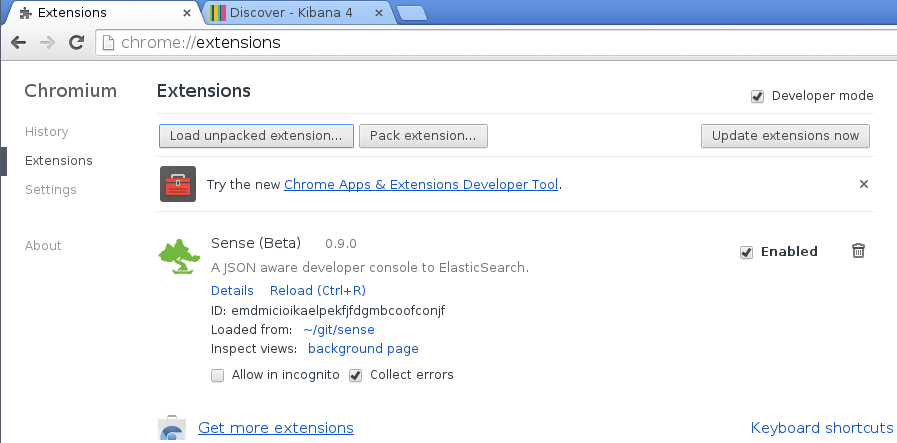
\includegraphics[width=12cm]{senseinstall.png}
\label{fig:senseinstall}
\caption{Plugin Sense installé dans chromium}
\end{figure}

Et voilà ! \footnotesize{(avec un accent anglais)}

\subsection{Utilisation de Sense}
L'utilisation de Sense est assez simple via son interface :

\begin{figure}[H]
\center
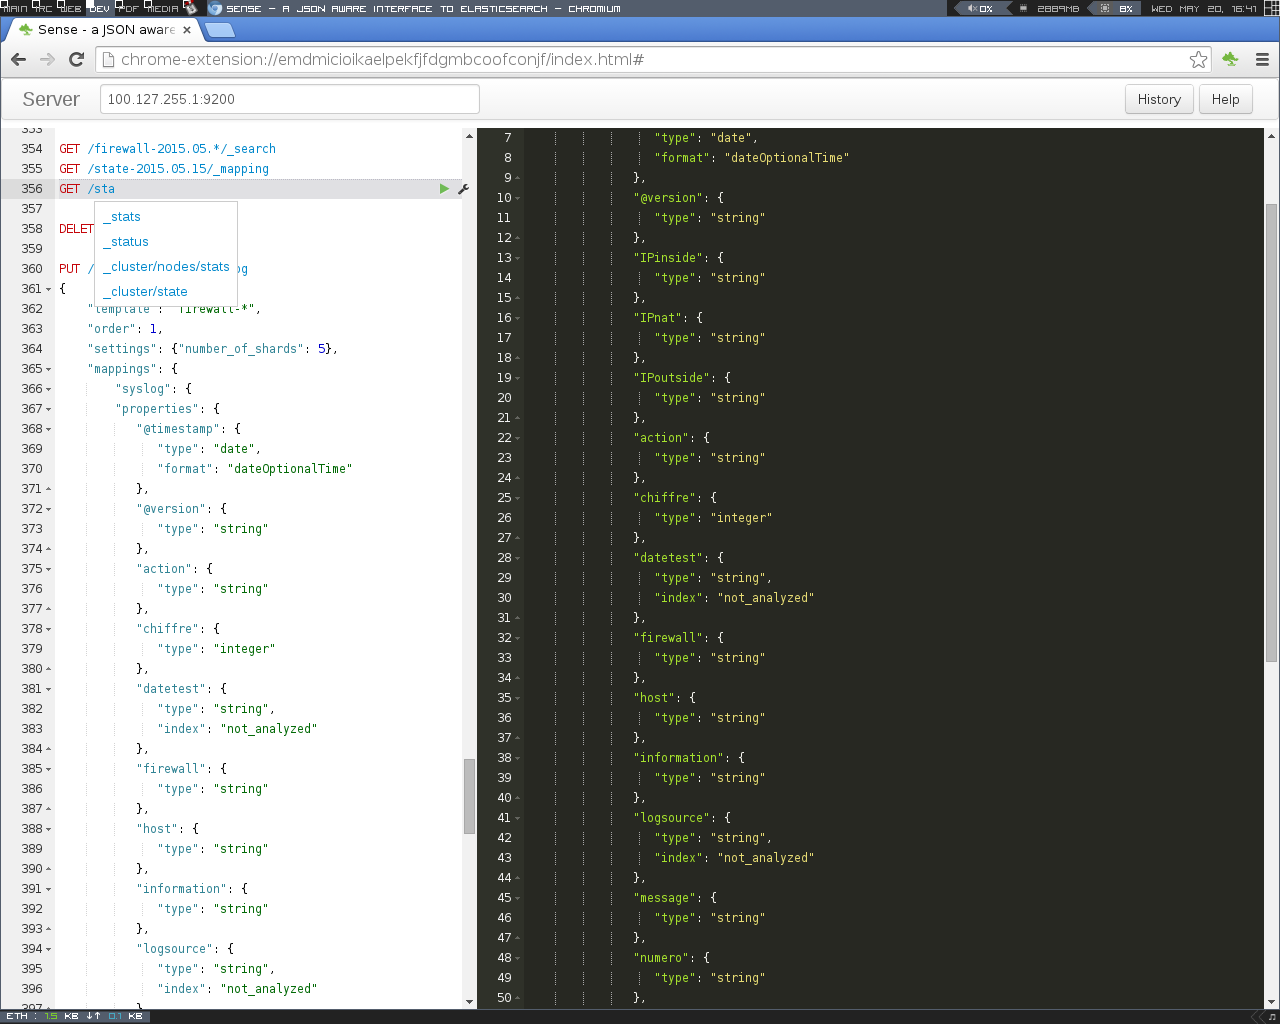
\includegraphics[width=15cm]{sensegui.png}
\label{fig:sensegui.png}
\caption{Vue générale de Sense}
\end{figure}

La difficulté se situe évidemment plutôt du coté de l'appréhension, la configuration
et l'optimisation de Elasticsearch.

Nous allons avec l'image ci-dessous \ref{fig:sensegui2.png} brièvement expliquer le fonctionnement de Sense
\begin{figure}[H]
\center
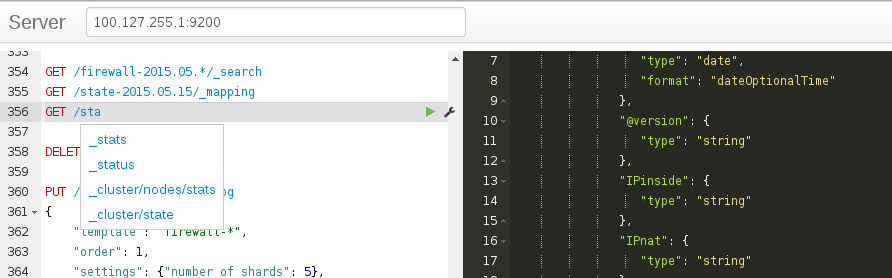
\includegraphics[width=15cm]{sensegui2.png}
\label{fig:sensegui2.png}
\caption{Zoom sur les fonctionnalités de Sense}
\end{figure}
Le formulaire \textbf{Server} situé en haut correspond à l'adresse et au port d'écoute 
de l'instance Elasticsearch sur laquelle on souhaite travailler.

Le panneau de gauche correspond au \textbf{panneau de requête}. On utilise l'api REST d'elasticsearch
pour envoyer des requêtes (recherches, modification etc, point sur l'API prévu 
ultérieurement). Il est à noté que le panneau de gauche est doté d'une autocomplétion
pour les fonctions et configurations standards dans elasticsearch.

Le panneau de droite est le \textbf{panneau de réponse} aux requêtes. Les informations
nous parviennent en JSON.

\section{La théorie}

\subsection{Approximation et comparaison avec le modèle relationnel}
La comparaison entre Elasticsearch et une base de données n'est pas forcement heureuse,
c'est un moteur de recherche (d'indexation). Il utilise donc la notion d'index   
qu'on peut cependant assez facilement comparer au modèle relationnel.

Elasticsearch s'organise autour d'index que l'on peut comparer aux bases (de données)
dans le modèle relationnel, un index peut utiliser plusieurs types (dans notre projet
nous aurions pu différencier les logs firewall des logs \textit{states} en utilisant 
les types), les types s'apparentent aux tables dans le modèle relationnel. 
Chaque enregistrement d'Elasticsearch est effectué sous forme document. Les documents
(qui ont un type, éventuellement type par défaut), un document peut être comparé 
à une ligne, ou un enregistrement. Ces lignes sont constitués de colonnes, appellées
champs (ou fields) dans Elasticsearch.


{\Huge NEED image}


\section{L'infrastructure}

\subsection{Le tunning}
Voici quelques conseilles qui sont applicables pratiquement dans toutes les situations
pour une utilisation optimale de Elasticsearch.

\subsubsection{Ne pas utiliser la swap}
Il est très fréquent (et souvent nécessaire) de formater une partition de swap pour
que le système puisse optimiser son fonctionnement. C'est très pratique pour ne pas
saturer la mémoire RAM de nos machines de bureau, notamment quand on voit la consommation
pantagruélique de certains navigateurs internet récents. Les fichiers qui ne sont 
susceptible de ne pas être utilisé avant un long moment sont parfois stocké sur le
disque dur afin de libérer de l'espace pour d'autres applications, la swap est
également utilisé lorsque l'on met un ordinateur en veille \ldots

La situation n'est pas la même sur un serveur. Ici nous sommes relativement maitre
de notre environnement, et de plus nous voulons que le service Elasticsearch soit 
le plus véloce possible, pour se faire il faut au contraire l'empêcher au maximum 
d'utiliser la partition de swap (forcément plus lente).

Il existe plusieurs façon de faire (y compris ne pas utiliser de partition de swap)
celle que j'ai choisie d'utiliser est de modifier la variable \ipath{vm.swapiness}
dans le fichier \ipath{/etc/sysctl.conf}. La swapiness représente le pourcentage
de mémoire RAM restant à partir duquel on commence à envoyer de informations en
swap.

\begin{lstlisting}[style=code,label={lst:configswapiness},caption={Configuration swapiness}]
vm.swapiness = 2
swapoff -a
swapon -a
\end{lstlisting}
Il existe deux méthodes pour que le changement de swapiness soit pris en compte :
redémarrer la machine ou bien désactiver puis réactiver la swap, via les commandes
swapon, swapoff. Utiliser la commande swapoff est également une mesure radicale à 
notre problème.

\subsubsection{Utiliser une quantité de RAM raisonné}
Elasticsearch est limité par Java. Avant de parler de ces limites, il faut rappeler 
que Elasticsearch est un front-end à Apache Lucene. Lucene est conçu pour tirer 
parti très efficacement du cache des système de fichiers (probablement ext4 si 
vous utilisez Debian), qui sont en définitif, gérer par le 
noyau\footnote{https://www.elastic.co/guide/en/elasticsearch/guide/current/\_limiting\_memory\_usage.html}.
Il est conseillé par la documentation de donner au maximum 50\% de la mémoire RAM
disponible à Elasticsearch, le reste étant dévouer à lucène et au bon fonctionnement
du système.
Dans notre installation dont nous parlerons plus en détail ultérieurement, nous 
avons choisi de nous réserver une bonne marge de manœuvre puisqu'un redis et un Logstash
minimalistes tournent en sus sur la machine hébergeant Elasticsearch.

Cependant cette valeur de 50\% n'a de sens que si Elasticsearch consomme moins de 
32Go de RAM, en effet, en allouer plus devient contreproductif puisque jusqu'à 32Go
la machine virtuelle Java (JVM) \textit{compresse} les adresses des pointeurs, 
(tant qu'on reste sous la limite des 32Go de RAM on peut continuer à utiliser les 
adresses mémoires sur 4 octets), après, la consommation de mémoire explose et le
\textit{garbage collector} devient bien moins efficace.

Pour les machines possédant une énorme quantité de mémoire RAM (128Go à 1To)
il conseiller pour optimiser le fonctionnement de la machine de faire tourner plusieurs
noeuds d'Elasticsearch dessus (attention aux entrées sortie et à l'utilisation processeur).

\subsection{Faire du nettoyage régulièrement}
Plus Elasticsearch agrège des données plus il s'empâte, ce phénomène est inévitable 
sur le long terme. Les contre-mesures sont de scale-out (monter à l'échelle horizontalement)
en rajoutant de nouveaux nœuds à notre cluster elastic search. On s'appliquera à 
manager les shards de façon optimisé bref à faire du fine tuning.

Pour éviter ce ralentissement la solution la plus radicale reste de supprimer les 
données. Justement, dans le cadre de notre projet, nous n'avons pas besoin de conserver 
toutes les données sur le long terme. Nous avons donc décider de supprimer les logs 
de changement d'état des par-feu tous les 4 jours. Ces logs peuvent représenter 
jusqu'à 30Go de données journalières. 
Pour ce faire nous utiliserons un tâche \textbf{cron} couplé à un script bash 
\ref{lst:scriptdelindex} tirant parti de l'API d'Elasticsearch dont nous parlerons 
plus bas. Pour indication, les index de firewall son supprimés tous les 4 jours, 
(une requête judiciaire/alerte sécurité arrive en général en moins de 3 jours).\\ 
Les logs sont de toute façon également conservés ailleurs pour se soumettre aux 
imperatifs judiciaires. Les index d'état (intéressants pour établir des statistiques)
sont conservés 1 mois.\\
Remarque sur la commande curl et son utilisation dans cron

\begin{lstlisting}[style=code,label={lst:curlexemple},caption={Extrait de notre script \ref{lst:scriptdelindex}}]
curl -sS -XDELETE $blade:$port/$target-$d
\end{lstlisting}

On remarque ici l'utilisation de l'option -sS pour \textit{silent, Show errors}.
Ainsi cron n'est pas importuné par les retour sur la sortie standard cela permet
également, en ajoutant la directive \textbf{MAILTO: mail@example.fr} de renvoyer
la sortie d'erreur vers mail@example.fr. Cela nécessite évidemment d'avoir configurer
un serveur mail sur notre machine, par défaut sur Debian, Exim (dpkg-reconfigure 
exim-config).

Concernant -XDELETE c'est une utilisation de l'API REST décrite plus bas.

Une des stratégies préconisé dans le cas où l'on souhaite conserver des données sur
le long terme alors qu'on en a seulement un besoin d'accès et d'analyse ponctuel ;
consiste à les enregistrer dans des fichiers séparés (output Logstash) et de les 
faire ingérer à un cluster Elasticsearch dimesinonné en conséquence le moment venu.



\section{Les API Elasticsearch}
Elasticsearch est énorme, mais être assez facilement utilisable par le 
plus grand nombre, des \gls{API} \emph{optimisées} pour chaque tâches ont été conçues.

\subsection{API REST}
Cette API sert à la communication avec Elastisearch, comme toutes les API REST elle
utilise les méthodes HTTP, ici : GET, POST, PUT et DELETE et s'appuie ensuite sur l'architecture d'Elasticsearch.

\textbf{{\color{grey}http://host:port}/[{\color{red}index}]/[{\color{cyan}type}]/[{\color{yellow}\_action/id}]}\\[5mm]
Imaginons que dans un projet fictif, nous souhaitions référencer des tweets.
On pourrait procéder comme suit pour ajouter le premier.

\textbf{PUT  {\color{grey} http://100.127.255.1:9200}/{\color{red}twitter}/{\color{cyan}tweet}/{\color{yellow}1}}

\begin{lstlisting}[style=code,label={lst:RESTexemple1curl},caption={Avec curl}]
curl -XPUT http://100.127.255.1:9200/twitter/tweet/1
\end{lstlisting}
Voici le résultat en utilisant curl, directement en ligne de commande, par 
navigateur, \ldots

\begin{lstlisting}[style=code,label={lst:RESTexemple1sense},caption={Avec Sense}]
PUT /twitter/tweet/1
\end{lstlisting}

Voici la syntaxe que nous obtiendrions en utilisant Sense, puisque notre serveur 
et notre port sont déjà renseignés, la syntaxe est bien plus courte.

La directive PUT est utilisé pour renseigner de nouvelles informations dans Elasticsearch.


Dans notre projet d'analyse de logs, il est fréquent que nous dussions supprimer 
des index, notamment dans le cas du paramétrage des \emph{mappings}, mais également
pour soulager notre infrastructure du poids des logs de firewall (~20-30Go/jours).\\

\textbf{DELETE  {\color{grey} http://100.127.255.1:9200}/{\color{red}twitter}/}\\

Si nous avions un index twitter journalier il serait possible d'utiliser une commande
très similaire pour supprimer tous les indexs d'un seul coup :\\

\textbf{DELETE  {\color{grey} http://100.127.255.1:9200}/{\color{red}twitter*}}\\

La directive DELETE est utilisé pour supprimer des informations d'Elasticsearch.\\


Enfin la directive GET qui sert à récupérer des information, à tout niveaux, index,
type, mapping, type par défaut \ldots, en revanche il faut avoir un identifiant exact,
ce n'est pas un outils de recherche (abordé dans la section suivante).\\[5mm]
\textbf{GET  {\color{grey} http://100.127.255.1:9200}/{\color{red}twitter}/{\color{cyan}tweet}/{\color{yellow}1}}\\

Les information récupérées le sont en JSON.

\subsection{Les API de recherche}
DSL pour Domain Specific Language, parce que Elasticsearch est avant tout un moteur 
de recherche, il dispose de puissantes fonctionnalités de recherche. Il dispose donc
de son propre langage d'interrogation le QueryDSL. C'est loin d'être un cas unique,
par exemple Puppet dispose également de son propre langage de configuration.

Il existe plusieurs API (ou méthodes) de recherche dans Elasticsearch nous les  
détaillerons plus en détail après avoir expliquer le fonctionnement général d'une
recherche dans Elasticsearch.

La recherche dans Elasticsearch est particulièrement efficace, car Elasticsearch 
indexe tout le contenu de ses documents (il indexe chaque field, en fonction d'un
mapping (discuté plus bas)).
C'est pour permettre l'indexation qu'Elasticsearch utilise du JSON structuré.



\subsubsection{Empty Search}
C'est la forme la plus basique de l'API de recherche, on ne spécifie pas de requête
spécifique. Comprendre le fonctionnement de cette API basique permettra d'utiliser
plus efficacement SearchLite, qui en est l'évolution directe.


\begin{lstlisting}[style=code,label={lst:APIsearchemptyexample1},caption={le "Hello World" de la recherche}]
GET /_search
\end{lstlisting}

Cette requête retourne tous les documents, de tous les index du cluster duquel nous
sommes membre.

\begin{lstlisting}[style=code,label={lst:APIsearchemptyexample2},caption={Réponse type à notre requête précédente}]
{
    "took": 798,
    "timed_out": false,
    "_shards": {
        "total": 201,
        "successful": 201,
        "failed": 0
    },
    "hits": {
        "total": 353585048,
        "max_score": 1,
        "hits": [
        {
            "_index": ".kibana",
            "_type": "visualization",
            "_id": "Top5-nat-firewall-router",
            "_score": 1,
            "_source": {
                "title": "Top5 nat-firewall router",
                "visState": "{\"type\":\"histogram\",\"params\":{\"shareYAxis\":true,\"addTooltip\":true,\"addLegend\":true,\"mode\":\"stacked\",\"defaultYExtents\":false},\"aggs\":[{\"id\":\"1\",\"type\":\"count\",\"schema\":\"metric\",\"params\":{}},{\"id\":\"2\",\"type\":\"terms\",\"schema\":\"group\",\"params\":{\"field\":\"IPnat\",\"size\":5,\"order\":\"desc\",\"orderBy\":\"1\"}}],\"listeners\":{}}",
                "description": "",
                "version": 1,
                "kibanaSavedObjectMeta": {
                "searchSourceJSON": "{\"index\":\"firewall-*\",\"query\":{\"query_string\":{\"query\":\"*\",\"analyze_wildcard\":true}},\"filter\":[]}"
                }
            }
        },
        .... REMOVED ...
    }
}
\end{lstlisting}

\paragraph{hits}
Hits représente le nombre total de documents retournés, ici 353585048, c'est le
nombre de résultats.
\paragraph{took}
Took est le temps en millisecondes pris pour effectué cette requête, ici 798
\paragraph{shard}


\subsubsection{SearchLite}

\subsubsection{Full-Body Search et QueryDSL}

\section{Le mapping}



\part{Annexes}
\chapter{Sources/Webographie/Bibliographie}
Web
Introduction généraliste à ELK \\

https://wooster.checkmy.ws/2014/04/elk-elasticsearch-logstash-kibana/

Explications sur les moteurs d'indexation/elasticsearch\\
https://zestedesavoir.com/articles/120/elasticsearch-maintenant-en-version-14/



Documentation de logstash\\
http://logstash.net/docs/1.4.2/
http://logstash.net/docs/1.4.2/flags

Installation de logstash
http://www.elastic.co/guide/en/elasticsearch/reference/1.4/setup-repositories.html
\\ et un peu d'astuce ou bien \\
https://github.com/elastic/logstash
\\ et un peu d'huile de coude


Debugger pour le filtre grok
http://grokdebug.herokuapp.com/


Documentation d'Elasticsearch\\
http://www.elastic.co/guide/en/elasticsearch/reference/current/index.html\\
http://www.elastic.co/guide/en/elasticsearch/guide/current/index.html



Documentation de Kibana
http://www.elastic.co/guide/en/kibana/current/
https://github.com/elastic/kibana/tree/master/docs


Livres\\
The logstash book
http://www.logstashbook.com/

Rapport projet tutoré ASRALL sur les MOM
http://webloria.loria.fr/~lnussbau/ptasrall2015/rapport\_a\_mom.pdf


Vidéos
Conférence de Jean Baptiste Favre, architecte réseau de blablacar.fr, à PSES 2014\\
http://numaparis.ubicast.tv/videos/kibana/



\begin{lstlisting}[style=code]
CREATE USER 'root'@'192.168.1.28' IDENTIFIED BY 'pomme';
CREATE USER 'root'@'192.168.1.28' IDENTIFIED BY 'pomme';
CREATE USER 'root'@'192.168.1.28' IDENTIFIED BY 'pomme';CREATE USER 'root'@'192.168.1.28' IDENTIFIED BY 'pomme';
Pommeeee carton pate
IO pome IO la pomee de'io
\end{lstlisting}

pommeepompompomo

\begin{lstlisting}[style=code]
#!/usr/bin/ruby

sfile=ARGV[0]
dfile=ARGV[1]

IO.readlines(sfile).each {|line|
`echo "#{line}" >> #{dfile}`
}
\end{lstlisting}

\printglossaries

\end{document}
